\documentclass[a4paper,12pt]{book}

\usepackage[utf8]{inputenc}
\usepackage[T1]{fontenc}
\usepackage[french]{babel}
\usepackage{geometry}
\usepackage{hyperref}
\usepackage{graphicx}
\usepackage{listings}
\usepackage{amsmath}
\usepackage{chngcntr}

\counterwithin{figure}{section} % numérotaion auto des figures en fonction de la section
\graphicspath{{images/}} % Set du dossier des images
\allowbreak 
\geometry{ % les marges
  left=1.5cm,
  right=1.5cm,
  top=2cm,
  bottom=1.5cm
}

\title{Rapport technique\\Véhicule autonome omnidirectionnel}
\author{Cyprien Siaud}
\date{\today}

\begin{document}

% \maketitle


\begin{titlepage}
    \centering

    % Logos
    
\includegraphics[width=4cm]{logo.png}
    \vspace{1em}

    % Titre
    {\Huge\bfseries Voiture Autonome Omnidirectionnelle\par}
    \vspace{0.5em}

    {\Large Rapport de Conception et Développement\par}
    \vspace{1.5em}

    % Image principale
    % \includegraphics[width=0.8\textwidth]{car/nice.jpg}
    \vspace{1.5em}
    \newpage

    % Informations générales
    \begin{tabular}{rl}
        Auteur : & Cyprien Siaud \\
        Date de début : & 18/06/2025 \\
        Date de fin : & ??/??/???? \\
    \end{tabular}

    \vfill

    % Résumé court
    \begin{minipage}{0.85\textwidth}
        \centering
        Ce rapport présente la conception, le développement et les tests d'une voiture autonome omnidirectionnelle capable de se déplacer librement dans toutes les directions grâce à un système de roues omnidirectionnelles et à une architecture de navigation autonome.
        
        \vspace{2em}

        Ce projet a pour objectif la participation à la Tiny Toulouse Robot Race (Tiny TRR) 2027, une compétition de robotique autonome où des véhicules miniatures doivent parcourir un circuit prédéfini le plus rapidement possible sans intervention humaine. La conception du véhicule vise à optimiser la vitesse, la précision de navigation et la fiabilité du système dans des conditions réelles de course.
    \end{minipage}

    \vfill

    % {\large \today\par}

\end{titlepage}

% =========================================================

\tableofcontents
% \newpage

% =========================================================
\chapter{Introduction}

% =========================
\section{Règlement de la Tiny TRR (Toulouse Robot Race)}
La Tiny Toulouse Robot Race (Tiny TRR) est une course de vitesse destinée à des petits robots autonomes, le vainqueur sera celui qui aura obtenu le meilleur temps sur un parcours prédéfini.
\vspace{1em}

\textbf{Les véhicules sont répartis en 3 catégories :}

\begin{itemize}
  \item Les "Roulants"
  
  Les robots de cette catégorie doivent être mus par des roues ou des sphères. Les robots peuvent avoir une ou plusieurs roues (sphères), motorisées ou non. Les véhicules à chenilles et les aéroglisseurs sont également rangés dans cette catégorie.
  \item Les "Piétons"
  
  Les robots de cette catégorie ne peuvent avoir, au maximum, que deux points d’appui (pieds) avec le sol (roues et sphères interdites).
  \item Les "Multi pattes"
  
  Les robots peuvent avoir un nombre illimité de points d’appui (« pattes » au sens large, etc.) avec le sol (roues et sphères interdites). Plus généralement, cette catégorie regroupe tous les robots ne rentrant pas dans l’une des deux premières catégories. Les drones volants sont exclus de la compétition.
\end{itemize}
\vspace{1em}

Les robots doivent concourir aux épreuves de manière totalement autonome. Ils doivent donc être guidés et pilotés uniquement par des systèmes embarqués, sans aide d’un système externe.
\vspace{1em}

Ils pourront se guider à l’aide de n’importe quel type de capteur embarqué (tactile, laser, ultra son, imagerie, …), qui devront donc être placés sur le robot lui-même et dont les signaux devront être produits et traités par le robot seul.

% -------------------------
\subsection{La sécurité}
Les moteurs et turbines thermiques, les systèmes pyrotechniques et les êtres-vivants sont interdits à bord des véhicules.
\vspace{1em}

Les robots doivent être munis d’un dispositif d’arrêt d’urgence (interrupteur poussoir rouge, interrupteur avec manche de 5 cm, …) facilement accessible. En cas de dispositif d’arrêt d’urgence télécommandé, la télécommande sera remise au juge avant le départ de chaque manche.
\vspace{1em}

\newpage
% -------------------------
\subsection{Procédure de départ}

Les procédures de départ doivent être respectées sous peine de pénalité de temps.
\vspace{1em}

Une fois le robot positionné sur la piste, seules les actions suivantes sont autorisées avant le départ :

\begin{itemize}
    \item La mise sous tension du robot
    \item Les réglages effectués par une seule personne, dans une limite de temps de 3 minutes
\end{itemize}

Lorsque le robot est prêt à prendre le départ, le concurrent en informe le chronométreur. Celui-ci annonce alors : \og PRÊT ? \fg.

À partir de ce moment, le concurrent peut déclencher le départ du robot à l'aide du dispositif de son choix : bouton poussoir, câble à éjecter, télécommande, \dots

Le démarrage peut être immédiat ou différé par une temporisation maximale de 5 secondes. Dès l'activation du départ, le concurrent doit quitter immédiatement la piste. Le chronométreur déclenche son chronomètre dès que le robot commence à se déplacer.

% -------------------------
\subsection{Arrivée}

Le chronomètre sera arrêté quand le robot franchira la ligne d’arrivée.
Le robot devra s’arrêter de manière autonome avant la fin du 6ième tour.

En cas d’arrêt non automatique, le juge/arbitre arrêtera le robot et une pénalité de 2 minutes sera appliquée.

% -------------------------
\subsection{La Piste}

La piste, d’une largeur de 1 mètre, s’inscrit dans un rectangle de dimensions 10 × 5 m. Les robots y évoluent dans le sens horaire. La longueur d’un tour de piste est de 24,30 m.

Les bordures sont disposées sur une bâche en PVC.

La piste centrale est constituée d’une sérigraphie noire de 5 cm de large, délimitant une ligne centrale blanche de 5 cm. Elle se compose d’une succession de segments droits et de virages. Tous les virages possèdent un rayon de courbure central de 1 mètre.

\begin{figure}[h]
    \centering
    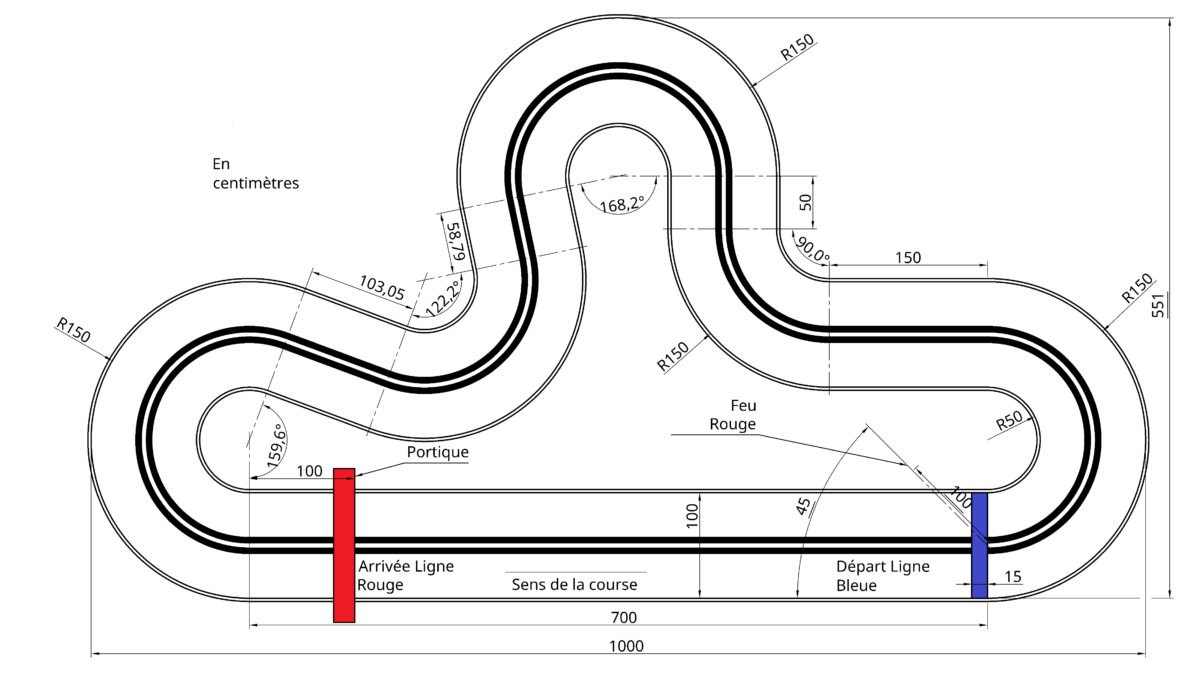
\includegraphics[width=0.75\textwidth]{piste.png}
    \caption{Plan de la piste}
    \label{fig:mesh}
\end{figure}

% =========================
\section{Objectif du Projet}

L’objectif final est simple : remporter la course.

Au-delà de cet objectif compétitif, le projet vise principalement la conception et le développement d’un véhicule autonome. Celui-ci sera équipé d’un lidar, de capteurs de ligne, ainsi que de roues omnidirectionnelles de type mecanum, permettant une grande liberté de mouvement.

% =========================
\section{L'équipe}

Bien que ce véhicule soit principalement conçu par mes soins (Cyprien Siaud), il s’inscrit dans une démarche collective, regroupant et capitalisant le savoir-faire du Montaulab.
\vspace{1em}

\textbf{Les principaux contributeurs du projet sont les suivants :}
\begin{itemize}
  \item Cyprien Siaud : conception et assemblage de la structure, intégration du véhicule et développement du logiciel du contrôleur
  \item Sébastien Duboisset : supervision du projet, formation et accompagnement à la fabrication de la batterie
  \item Jean-Claude Viala : assistance dans le choix des composants électroniques
  \item Philippe Bonnaud : contribution à la conception de la structure mécanique
  \item Arnaud Boëlle : aide à l’analyse des problématiques physiques, électroniques et algorithmiques
\end{itemize}

Chacun de ces contributeurs étant également participant à la course, l’esprit de compétition est naturellement présent et constitue un facteur de motivation supplémentaire.

% =========================
\section{Composition du véhicule}

Le véhicule est composé de deux ensembles complémentaires : la partie mécanique et la partie électronique, formant un système unique une fois assemblés.
\vspace{1em}

\textbf{Partie mécanique :}
\begin{itemize}
  \item un châssis en profilé aluminium de 30 mm de largeur, intégrant un pivot central permettant une rotation relative entre l’avant et l’arrière du véhicule
  \item quatre roues omnidirectionnelles de type mecanum
  \item quatre moteurs permettant le contrôle indépendant de chaque roue
\end{itemize}

\vspace{1em}

\textbf{Partie électronique :}
\begin{itemize}
  \item un lidar rotatif 360° pour l’analyse des bords de piste ;
  \item deux capteurs de ligne permettant de distinguer le noir du blanc afin de maintenir l’alignement au centre de la piste ;
  \item une carte Arduino DUE offrant une puissance de calcul supérieure à une carte Arduino classique ;
  \item deux contrôleurs de puissance assurant l’alimentation des quatre moteurs ;
  \item un module ESP32 (Wi-Fi) permettant une interface de contrôle et de supervision du véhicule.
\end{itemize}

% =========================================================

\chapter{Composants matériel}
% =========================================================

\section{la structure}

Réalisée à l'aide de profilés aluminium de 30x30mm la structure est composée de 2 parties maintenues ensembles par un palier et une tige filetée.


\end{document}